% Options for packages loaded elsewhere
\PassOptionsToPackage{unicode}{hyperref}
\PassOptionsToPackage{hyphens}{url}
\PassOptionsToPackage{dvipsnames,svgnames,x11names}{xcolor}
\documentclass[
  11pt,
  a4paper,
]{article}
\usepackage{xcolor}
\usepackage[margin=23mm]{geometry}
\usepackage{amsmath,amssymb}
\setcounter{secnumdepth}{-\maxdimen} % remove section numbering
\usepackage{iftex}
\ifPDFTeX
  \usepackage[T1]{fontenc}
  \usepackage[utf8]{inputenc}
  \usepackage{textcomp} % provide euro and other symbols
\else % if luatex or xetex
  \usepackage{unicode-math} % this also loads fontspec
  \defaultfontfeatures{Scale=MatchLowercase}
  \defaultfontfeatures[\rmfamily]{Ligatures=TeX,Scale=1}
\fi
\usepackage{lmodern}
\ifPDFTeX\else
  % xetex/luatex font selection
  \setmainfont[BoldFont=texgyrepagella-bold.otf,ItalicFont=texgyrepagella-italic.otf,BoldItalicFont=texgyrepagella-bolditalic.otf]{texgyrepagella-regular.otf}
  \setmonofont[]{lmmono10-regular.otf}
  \setmathfont[]{texgyrepagella-math.otf}
\fi
% Use upquote if available, for straight quotes in verbatim environments
\IfFileExists{upquote.sty}{\usepackage{upquote}}{}
\IfFileExists{microtype.sty}{% use microtype if available
  \usepackage[]{microtype}
  \UseMicrotypeSet[protrusion]{basicmath} % disable protrusion for tt fonts
}{}
\makeatletter
\@ifundefined{KOMAClassName}{% if non-KOMA class
  \IfFileExists{parskip.sty}{%
    \usepackage{parskip}
  }{% else
    \setlength{\parindent}{0pt}
    \setlength{\parskip}{6pt plus 2pt minus 1pt}}
}{% if KOMA class
  \KOMAoptions{parskip=half}}
\makeatother
\setlength{\emergencystretch}{3em} % prevent overfull lines
\providecommand{\tightlist}{%
  \setlength{\itemsep}{0pt}\setlength{\parskip}{0pt}}
\usepackage{mathtools}
\usepackage{graphicx}
\usepackage{needspace}
\usepackage{xurl}
\usepackage{etoolbox}
\usepackage{fancyhdr}
\usepackage{titlesec}
\setlength{\parindent}{0pt}
\setlength{\parskip}{5.5pt plus 1pt minus 1pt}
\setlength{\emergencystretch}{2em}
\clubpenalty=10000
\widowpenalty=10000
\displaywidowpenalty=10000
\raggedbottom
\pagestyle{fancy}
\fancyhf{}
\fancyfoot[C]{\small\thepage}
\renewcommand{\headrulewidth}{0pt}
\titleformat{\section}{\normalfont\Large\bfseries}{}{0pt}{}
\titlespacing*{\section}{0pt}{16pt plus 3pt minus 2pt}{7pt}
\pretocmd{\section}{\Needspace{6\baselineskip}}{}{}
\pretocmd{\subsection}{\Needspace{5\baselineskip}}{}{}
\makeatletter
\renewenvironment{figure}[1][]{\par\noindent\begin{minipage}{\linewidth}\def\@captype{figure}}{\end{minipage}\par\medskip}
\def\@maketitle{\newpage\null\begin{center}{\LARGE\bfseries\@title\par}\vskip .9em{\large\@author\par}\vskip .5em{\small\@date\par}\end{center}\vskip .4em}
\makeatother
\newsavebox{\papereqbox}
\newcommand{\paperdisplay}[2][]{\par\begingroup
\sbox{\papereqbox}{$\displaystyle #2$}
\typeout{PAPER-EQUATION-WIDTH: \the\wd\papereqbox; available \the\linewidth; tag #1}
\begin{equation*}\ifdim\wd\papereqbox>.93\linewidth
\resizebox{.93\linewidth}{!}{\usebox{\papereqbox}}\else\usebox{\papereqbox}\fi
\ifstrempty{#1}{}{\tag{#1}}\end{equation*}\endgroup\par}
\usepackage{bookmark}
\IfFileExists{xurl.sty}{\usepackage{xurl}}{} % add URL line breaks if available
\urlstyle{same}
% fallback for those not using the hyperref driver hyperxmp:
\makeatletter
\@ifundefined{xmpquote}{\newcommand{\xmpquote}[1]{#1}}{}
\makeatother
\hypersetup{
  pdftitle={Transverse Chirality{,} Dihedral Harmonic Selection{,} and Local Linearization in a Three-Channel Nonlinear Map},
  pdfauthor={Hilmir Frímann Halldórsson},
  colorlinks=true,
  linkcolor={MidnightBlue},
  filecolor={Maroon},
  citecolor={Blue},
  urlcolor={MidnightBlue},
  pdfcreator={LaTeX via pandoc}}

\title{Transverse Chirality, Dihedral Harmonic Selection, and Local Linearization in a Three-Channel Nonlinear Map}
\author{Hilmir Frímann Halldórsson}
\date{25 September 2026}

\begin{document}
\maketitle

\section{Abstract}\label{abstract}

We study the direction of the raw channel chirality of the three-channel map defined in Paper A, using the observable and channel-transformation convention of Paper B. Near the synchronized unit-amplitude circle, the two transverse phase directions have the same linear multiplier. Nonlinear angular motion is nevertheless permitted because channel permutation symmetry is discrete. We derive the induced dihedral action, distinguish its oriented and projective isotropy classes, and show that the first possible in-plane angular term for a purely imaginary transverse seed has the form \(h^4\sin6\phi\). A complete coefficient recurrence proves this law for every finite update number. Its increment is a combination of four exponential rates, from which we obtain a parameter-dependent finite sum and limiting coefficient. At the historically selected parameters \(\epsilon=1/20,\ g=1/5\), the limiting coefficient is exactly \(13375/1107936648\). At \(\epsilon=1/20,\ g=1/5\), an all-degree valuation argument proves nonresonance of the five-dimensional gauge-fixed spectrum; the parameter-general local theorem assumes nonresonance. Established analytic-linearization theory then identifies the observed local angular change as a finite coordinate displacement, rather than attraction toward six preferred axes. We also derive the first-order change caused by the actual amplitude-then-phase composition. The historical seed and an existing two-seed experiment are explanatory examples, not premises of the general theorem. No physical gate, shell-coordinate or energy interpretation is established.

\section{1. Scope, provenance and the mathematical object}\label{scope-provenance-and-the-mathematical-object}

The recurrence is adopted from Paper A {[}PA, §§1,6.1{]}. The raw chirality and its channel transformation law are adopted from Paper B {[}PB, §§6--8{]}. This paper analyzes those definitions; it introduces no new runtime evolution law.

``Transverse'' here means transverse to the common-channel direction inside a three-channel state. Paper A also studies directions normal to a three-periodic sector of a twelve-site ring. That larger-ring normal space is a different object. Its numerical multipliers are not imported into the present theorem.

We use the ideal real-arithmetic equations. In particular, the recorded decimal parameter choices .05 and .2 are interpreted as the exact rationals \(1/20\) and \(1/5\) when proving the arithmetic corollaries. The accepted NumPy implementation evaluates the same formulas with binary64 coefficients and rounded arithmetic. The Poincare theorem and the prime-valuation proof are statements about the analytic mathematical map, not about a discontinuous rounding operation or a bitwise orbit.

The original rationale for the historically selected values
\paperdisplay[]{\epsilon=.05,\qquad g=.2,\qquad
\Omega_{\rm hist}=(.2+.3i,-.4+.1i,.1-.2i)^T}
remains unresolved. They are not labelled test-only, tuned or physically derived. Parameter-dependent formulas precede every specialization. Their earliest uses located in the bounded reconstruction, and precise unresolved questions, are recorded separately {[}S:Census, S:Questions{]}. An explicit input need not have a recovered physical motivation for its conditional mathematics to be analyzed.

The twelve \textbf{oriented} roots of \(\sin6\phi=0\) have three \(D_3\) orbits. Two types are obtained under \(D_6\), or on projective axes under \(D_3\). Section 6 proves these counts directly. The supplementary reconstruction record documents the calculation\textquotesingle s development and attribution. No novelty or priority claim is made for standard representation theory, polynomial identities or analytic linearization.

The local Poincare normal form is linear under the stated nonresonance hypotheses; the finite coefficient system below is a Taylor-jet calculation.

\section{2. Recurrence, notation and synchronization}\label{recurrence-notation-and-synchronization}

Let \(e=(1,1,1)^T\) and use the negative graph-Laplacian convention
\paperdisplay[1]{L_3=ee^T-3I=
\begin{pmatrix}-2&1&1\\1&-2&1\\1&1&-2\end{pmatrix}.}
The real parameters \(\epsilon,g,\lambda\) are respectively the amplitude coefficient, linear coupling coefficient and phase strength. In this paper the amplitude-coefficient triple is explicitly \(k=(1,1,1)\), an equal-unit special case of {[}PA{]}. The update is
\paperdisplay[2]{\widetilde\Omega_j=
\Omega_j+\epsilon\Omega_j(1-|\Omega_j|^2)+g(L_3\Omega)_j,}
followed simultaneously by
\paperdisplay[3]{p_j=\operatorname{Arg}_0(\widetilde\Omega_j),\quad
H_j(p)=\sum_{l\ne j}\sin(3(p_l-p_j)),\quad
\Omega_j^+=|\widetilde\Omega_j|e^{i[p_j+\lambda H_j(p)]}.}
The source convention is \(\operatorname{Arg}_0(0)=0\); at \(\lambda=0\) the phase step is directly the identity. Near the fixed state \(e\), all pre-sync components are nonzero and a smooth phase chart exists. We do not extend a local differentiability assertion through the source\textquotesingle s generally discontinuous nonzero-\(\lambda\) zero-amplitude stratum.

The coefficient three in (3) is part of the adopted model. Symmetry describes its consequences; it does not establish why the historical model selected it. There is no physical time scale implicit in the integer update number \(n\).

\textbf{Proposition 1 (synchronization and linear channel splitting).} The manifold \(\Omega=we\), \(w\in\mathbb C\), is invariant. The real plane
\paperdisplay[4]{V=e^\perp=\{z\in\mathbb R^3:e^Tz=0\}}
has \(L_3|_V=-3I\), while \(L_3e=0\).

\emph{Proof.} Since \(e^Te=3\), both linear identities follow from (1). Equation (2) maps \(we\) to \([1+\epsilon(1-|w|^2)]we\). Equal nonzero phases have zero increments in (3); common zero stays zero under the stated convention. In particular, \(|w|=1\) is a fixed circle, and \(e\) is its real representative. The radius one follows from the chosen unit value of \(k\); it is not a physical length or energy normalization. \(\square\)

Define the three local multipliers
\paperdisplay[5]{a=1-3g,\qquad r=a-2\epsilon,\qquad m=1-2\epsilon=1-a+r.}
Here \(a,r,m\) are derived multipliers, not additional model parameters. Their Jacobian derivation appears in §9.

Use the positive orthonormal basis
\paperdisplay[6]{u=\frac{(1,-1,0)^T}{\sqrt2},\qquad
v=\frac{(1,1,-2)^T}{\sqrt6},\qquad
\widehat e=\frac e{\sqrt3},\qquad u\times v=\widehat e.}
The square roots are the Euclidean lengths of the displayed integer vectors. Direct dot products verify transversality and orthonormality. Set
\paperdisplay[7]{q(\phi)=u\cos\phi+v\sin\phi,\quad q_\perp(\phi)=q(\phi+\pi/2),\quad
e\times q=\sqrt3q_\perp.}
The principal seed family is
\paperdisplay[8]{\Omega_0=e+i hq(\phi),\qquad h>0\ \text{sufficiently small}.}
The seed parameter \(h\) is a perturbation amplitude; \(\phi\) is an intrinsic channel angle. Neither is an external observer clock.

\section{3. Chirality and the exact plane decomposition}\label{chirality-and-the-exact-plane-decomposition}

For real channel vectors \(x=\Re\Omega,\ y=\Im\Omega\), Paper B defines
\paperdisplay[9]{C(\Omega)=x\times y.}
It is raw and unnormalized. It has no imposed decay envelope; it need not decay on general states or arbitrary dynamics. Decay in the local regime will be a consequence of the recurrence.

\textbf{Proposition 2.} If \(x=\alpha e+\xi,\ y=\beta e+\eta\), with \(\xi,\eta\in V\), then
\paperdisplay[10]{C=e\times(\alpha\eta-\beta\xi)+\xi\times\eta.}
The two terms are orthogonal: the first belongs to \(V\), the second to \(\mathbb Re\).

\emph{Proof.} Expand the cross product; \(e\times e=0\) and \(\xi\times e=-e\times\xi\). The first term has zero dot product with \(e\). If \(\xi,\eta\) are independent, they span the plane \(V\), so their cross product is normal to \(V\). If dependent, that product is zero, which also belongs to \(\mathbb Re\). Equivalently, substitution \(\xi=(x_1,x_2,-x_1-x_2)\), \(\eta=(y_1,y_2,-y_1-y_2)\) gives three equal cross-product components. \(\square\)

A common complex phase rotates the pair \((x,y)\) by a real two-dimensional matrix of determinant one and preserves \(x\times y\). Thus, for nonzero mean \(w=\frac13e^T\Omega\), rotate it to \(|w|>0\) and write
\paperdisplay[]{\Omega=|w|e+\xi+i\eta,\qquad \xi,\eta\in V.}
Then
\paperdisplay[]{C_\perp=|w|e\times\eta,\qquad C_\parallel=\xi\times\eta,}
\paperdisplay[11]{\frac{\|C_\parallel\|}{\|C_\perp\|}
\le\frac{\|\xi\|}{\sqrt3|w|}\quad(\eta\ne0).}
This proves plane approach under \textbf{relative} synchronization with nonzero common amplitude. Absolute approach to synchronized zero is insufficient: \(x=t(1,-1,0)\), \(y=t(1,1,-2)\) gives \(C=2t^2e\), longitudinal for every \(t\ne0\).

The raw channel triple is not automatically a vector in physical space. For a permutation matrix \(P\),
\paperdisplay[12]{C(P\Omega)=\det(P)PC(\Omega),\qquad
C(\overline\Omega)=-C(\Omega).}
The determinant in this channel pseudovector law is essential {[}PB, Proposition 5{]}.

\section{4. The historical directional observation as an example}\label{the-historical-directional-observation-as-an-example}

The recorded seed, rewritten exactly, is
\paperdisplay[13]{\Omega_{\rm hist}=(1/5+3i/10,-2/5+i/10,1/10-i/5)^T.}
Its selection rationale is OPEN. The following calculation concerns that explicitly supplied example only.

Its mean is \((-1+2i)/30\). Multiplication by
\paperdisplay[14]{Q=(-1-2i)/\sqrt5,\qquad |Q|=1}
makes the mean \(w=\sqrt5/30\). Direct multiplication gives
\paperdisplay[]{\xi=\sqrt5(7/150,13/150,-2/15)^T,\qquad
\eta=(7\sqrt5/50)(-1,1,0)^T.}
Consequently
\paperdisplay[15]{w e\times\eta=\frac7{300}(-1,-1,2)^T,\qquad
\xi\times\eta=\frac7{75}e,\qquad
C=(7/100,7/100,7/50)^T.}
Thus the reported transverse comparison direction is already encoded in the phase-rotated tangent component. It need not be invented as a universal nonlinear selector.

``First-order'' and ``second-order'' here describe dependence on transverse perturbations at fixed common component. They do not imply dominance in this finite seed: its relative distance is
\paperdisplay[16]{\frac{\sqrt{\|\xi\|^2+\|\eta\|^2}}{\sqrt3|w|}=2\sqrt5.}
Nor does the seed belong to the exact conjugate-swap invariant subspace below: its first two rotated real components differ.

If an orbit reaches the local synchronized regime, (11) explains why its longitudinal contribution becomes smaller than its transverse one. At first linear order the latter scales as \(a^n\), while the bilinear longitudinal term scales as \(r^na^n\). For the full local map, §11 proves the ratio bound \(O(r^n+a^{2n})\) under the analytic hypotheses, which is sufficient without identifying either expression with an exact finite-amplitude rate. This does \textbf{not} prove that (13) enters that local neighborhood or that its complete transient leaves the initial tangent direction unchanged. Its global basin and exact final axis remain outside the theorem.

\section{5. Dihedral action, polynomial invariants and harmonic selection}\label{dihedral-action-polynomial-invariants-and-harmonic-selection}

Let
\paperdisplay[]{P=\begin{pmatrix}0&0&1\\1&0&0\\0&1&0\end{pmatrix},\qquad
T=\begin{pmatrix}0&1&0\\1&0&0\\0&0&1\end{pmatrix}.}
In basis \((u,v)\),
\paperdisplay[17]{[P]_V=\begin{pmatrix}-1/2&-\sqrt3/2\\\sqrt3/2&-1/2\end{pmatrix},
\qquad [T]_V=\operatorname{diag}(-1,1).}
Thus \(P:\phi\mapsto\phi+2\pi/3\), \(T:\phi\mapsto\pi-\phi\), with \(P^3=T^2=I\), \(TPT=P^{-1}\). This faithful two-dimensional action of \(S_3\) on the complement of its trivial line is its standard representation. We use \(D_j\) for the planar dihedral group of order \(2j\): \(S_3\simeq D_3\).

Complex conjugation maps the seed (8) to the one with \(\phi+\pi\). It commutes with permutations. Its product with \(P^2\) rotates the circle by \(\pi/3\), so the extended seed-circle group is \(D_6\) of order twelve. Both (2) and the local form of (3) respect these operations: permutations relabel all pair differences, and conjugation reverses every phase and sine increment.

Write
\paperdisplay[18]{C_n=A_C q_\perp+B_C q+D_C\widehat e.}
Under a transposition, (12) makes \(A_C\) even and \(B_C,D_C\) odd in the reflected angle. Under conjugation \(A_C,B_C\) are unchanged and \(D_C\) reverses. Under \(P\) all three coefficients are periodic with \(2\pi/3\). It follows that the signed local angle
\paperdisplay[19]{\psi_n=\operatorname{atan2}(C_n\cdot(-q),C_n\cdot q_\perp)
=-\arctan(B_C/A_C)}
has only \(\sin(6j\phi)\) harmonics on its branch near zero. Positive angle uses the \(u\)-to-\(v\) orientation. Signed elevation permits \(\cos(3(2j+1)\phi)\). These restrictions concern the local branch where the direction is defined.

A polynomial argument identifies the lowest possible order without fitting. On \(q_1+q_2+q_3=0\), \(\sum q_j^2=1\), define
\paperdisplay[20]{I_3=\sum_jq_j^3=\frac{\sin3\phi}{\sqrt6},\qquad
\Delta=(q_1-q_2)(q_2-q_3)(q_3-q_1)
=\frac{\cos3\phi}{\sqrt2}.}
Therefore
\paperdisplay[21]{\sin6\phi=4\sqrt3\,I_3\Delta.}
An alternating polynomial vanishes on each equality line \(q_i=q_j\); the three distinct linear factors divide it, so \(\Delta\) divides it. The quotient is symmetric. A symmetric linear polynomial vanishes on the sum-zero plane. At symmetric cubic degree only one independent expression remains there: \(\sum q_j^3=3q_1q_2q_3\), while \(\sum_{i\ne j}q_i^2q_j=-\sum q_j^3\).

Write the chirality expansion as \(C(e+ihq)=\sum_k h^k c_k(q)\), allowing \(q\) to range over the full transverse plane \(V\). Each \(c_k\) is a homogeneous degree-\(k\) polynomial on \(V\), not merely a function on its unit circle. The polynomial \(c_k(q)\cdot q\) has degree \(k+1\). Its conjugation parity makes that degree even, and it is alternating under permutations. There is no such nonzero degree-two or degree-four polynomial. At degree six it is proportional to \(I_3\Delta\). Only after establishing these degree bounds do we restrict to \(\sum q_j^2=1\). Thus \(B_C\) first permits \(h^5\sin6\phi\), and division by the leading order-\(h\) chirality gives \(h^4\sin6\phi\). Longitudinal \(D_C\) is alternating and odd, so its first permitted term is degree three, proportional to \(\Delta\).

This separates \textbf{symmetry-forced harmonic/order restrictions} from \textbf{recurrence-specific coefficients}. Symmetry does not require every permitted coefficient to be nonzero.

\section{6. Exact one-step calculation and two isotropy types}\label{exact-one-step-calculation-and-two-isotropy-types}

Put \(s_2=q(\pi/2-2\phi)\), \(S=\sin3\phi\). Useful componentwise identities are
\paperdisplay[]{q^{\circ2}=e/3+s_2/\sqrt6,\quad q^{\circ3}=q/2+Se/(3\sqrt6),}
\paperdisplay[22]{q\circ s_2=q/\sqrt6+Se/3,\quad
s_2^{\circ2}=e/3-s_2/\sqrt6+\sqrt{2/3}Sq.}
At \(\lambda=0\), (2) applied to (8) gives exactly
\paperdisplay[]{\Re\Omega_1=e-\epsilon h^2q^{\circ2},\qquad
\Im\Omega_1=ahq-\epsilon h^3q^{\circ3}.}
Taking the cross product and projecting as in (18) yields
\paperdisplay[23]{\begin{aligned}
A_C&=\sqrt3h\left[a-\frac{\epsilon h^2(2a+3)}6+
\frac{\epsilon^2h^4(5+\cos6\phi)}{36}\right],\\
B_C&=\frac{\sqrt3}{36}\epsilon^2h^5\sin6\phi,\\
D_C&=\frac{\sqrt6}{12}\epsilon h^3(2a-\epsilon h^2)\cos3\phi .
\end{aligned}}
These are exact polynomial identities for the one pre-sync step, not asymptotic fits. For \(a>0\), the angle branch in (19) gives
\paperdisplay[24]{\psi_1=-\frac{\epsilon^2}{36a}h^4\sin6\phi+O(h^6),\qquad
\chi_1=\frac{\epsilon}{3\sqrt2}h^2\cos3\phi+O(h^4),}
where \(\chi=\operatorname{atan2}(C\cdot\widehat e,\|C_\perp\|)\) is signed elevation.

\textbf{Proposition 3 (isotropy types and the corrected orbit count).} The twelve oriented roots \(\phi=k\pi/6\) split as follows:
\paperdisplay[25]{\begin{array}{c|c}
D_3\text{ oriented orbit}&k\\ \hline
u\text{-type}&0,2,4,6,8,10\\
v\text{-type, first orientation}&3,7,11\\
v\text{-type, opposite orientation}&1,5,9
\end{array}}
The last two combine under conjugation to one \(D_6\) orbit. Projectively, \(k\) is taken modulo six and \(D_3\) has the two orbits \(\{0,2,4\}\), \(\{1,3,5\}\).

Thus the \(D_6\) orbits have sizes six and six, and the projective \(D_3\) orbits have sizes three and three. Each \(D_6\) orbit has a stabilizer of order two and is therefore not a regular orbit. The supplementary reconstruction record preserves the earlier terminology and its attributed correction.

\emph{Proof.} Apply \(k\mapsto k+4\) and \(k\mapsto6-k\) modulo twelve. Adding conjugation \(k\mapsto k+6\) combines the two three-element orbits. In particular \(T\) fixes \(v\), whose \(D_3\) stabilizer has two elements and whose orbit has three, not six, elements. \(\square\)

\begin{figure}
\centering
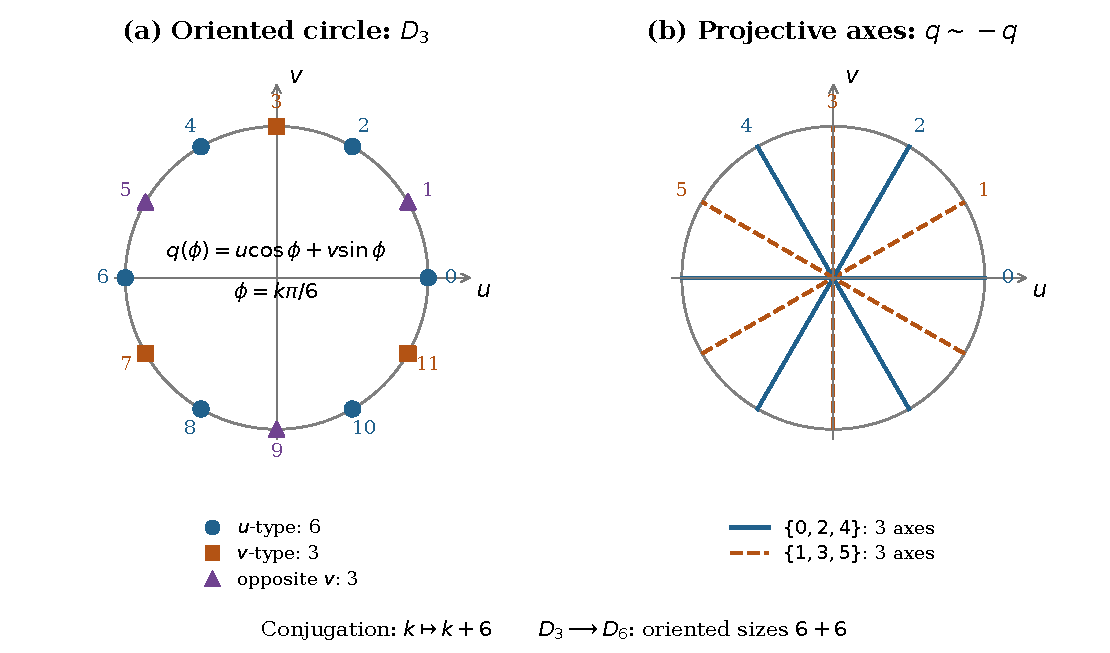
\includegraphics[width=\linewidth]{figures/figure_1_transverse_symmetry.pdf}
\caption{Intrinsic transverse symmetry. Left: the twelve roots \(\phi=k\pi/6\) on \(q(\phi)=u\cos\phi+v\sin\phi\), colored and shaped by the three \(D_3\) oriented orbits (sizes \(6,3,3\)). Right: antipodal identification gives the two projective classes, each with three axes; labels are \(k\bmod6\). Conjugation sends \(k\) to \(k+6\), joins the two oriented \(v\)-type orbits and extends the seed-circle action to \(D_6\). The \(D_6\) orbits have sizes \(6,6\), with stabilizers of order two. Coordinates are coefficients in the intrinsic \((u,v)\) basis, not physical-space coordinates.}
\end{figure}

The full-state stabilizers give stronger geometric constraints than the roots of a leading term alone. For \(u\)-type, conjugation followed by \(T\) fixes
\paperdisplay[26]{\Omega=(x+iy,x-iy,z),\quad x,y,z\in\mathbb R,\qquad
C=y(z,z,-2x).}
The transverse projection stays on the initial chirality line, but longitudinal elevation is allowed. For \(v\)-type, \(T\) fixes
\paperdisplay[27]{\Omega=(b+ic,b+ic,d+if),\quad b,c,d,f\in\mathbb R,\qquad
C=(bf-dc)(1,-1,0).}
This is a fixed transverse line. Equivariance preserves both fixed subspaces. The constraints are exact wherever the chirality direction is defined. Projective axes disregard a possible sign reversal; oriented zero-drift statements use the nonzero local branch. Neither subspace is being called an attractor.

If the transverse projection itself vanishes, its in-plane angle is undefined even when the total chirality is nonzero. The sufficiently small local seeds used in the angular theorems avoid that degeneracy.

The two chirality expressions (26)--(27) are orthogonal for arbitrary allowed amplitudes. The preserved experiment {[}S:AX{]} chose \(h=10^{-3}\), \(\epsilon=.05,g=.2,\lambda=0\), and recorded eight updates from each of \(e+ihu,e+ihv\). It has nine rows per seed. Its maximum recorded A-axis drift is \(1.1785113164\times10^{-8}\) rad, B-axis drift is zero, and the axes are measured at \(90^\circ\) at every row. The minimum norm is approximately \(1.1351167546\times10^{-6}\). These are binary64 observations; exact orthogonality comes from (26)--(27). This is a bounded falsification of unrestricted rapid universal-axis collapse, not a sample of generic directions. No trajectory is rerun for this paper.

\section{7. The arbitrary-step coefficient theorem}\label{the-arbitrary-step-coefficient-theorem}

We now derive the main zero-phase result without extrapolating a finite symbolic sequence.

\textbf{Theorem 4 (finite-step angular coefficient).} For the map (2), seed (8), \(\lambda=0\) and real \(\epsilon,g\), the coefficient recurrences below are polynomial recurrences with unrestricted \(r\). The division defining \(\kappa_n\) requires \(a\ne0\). With the additional condition \(a>0\), the chosen local signed-angle branch (19) has, for every fixed finite \(n\ge0\),
\paperdisplay[28]{\psi_n=\kappa_n(a,r)h^4\sin6\phi+O(h^6).}
The coefficient sequence has the recurrence and closed form below. Four distinct exponential rates describe its increments when the specified rate denominators are nonzero. This finite-\(n\) statement does not yet assert a remainder uniform in \(n\).

\emph{Proof.} Work before phase gauge fixing so that common modes are not discarded. Write
\paperdisplay[]{\Re\Omega_n=e+h^2x_n+h^4u_n+O(h^6),\quad
\Im\Omega_n=hy_n+h^3v_n+h^5w_n+O(h^7).}
Let \(L_Iz=az+(1-a)e(e^Tz)/3\), \(L_Rz=rz+(1-a)e(e^Tz)/3\).
Expansion of the source cubic gives
\paperdisplay[29]{\begin{aligned}
y'&=L_Iy,&x'&=L_Rx-\epsilon y^{\circ2},\\
v'&=L_Iv-\epsilon(2x\circ y+y^{\circ3}),\\
u'&=L_Ru-\epsilon(3x^{\circ2}+2y\circ v+x\circ y^{\circ2}),\\
w'&=L_Iw-\epsilon(2x\circ v+2u\circ y+x^{\circ2}\circ y+
3y^{\circ2}\circ v).
\end{aligned}}
All displayed terms are Taylor coefficients, not numerically evolved states.

Using (22), together with
\paperdisplay[]{q^{\circ5}=q/4+5Se/(18\sqrt6)+Ss_2/18,}
the coefficient space closes as follows. Each channel\textquotesingle s jet is polynomial in its own \(q_j\), with symmetric polynomial coefficients in the whole triple. On the full sum-zero plane, symmetric coefficients reduce to polynomials in \(\sum q_j^2\) and \(\sum q_j^3\). Restricting to the unit circle and reducing by \(t^3=t/2+S/(3\sqrt6)\) leaves the span of \(e,q,s_2\), with coefficients polynomial in \(S\). Homogeneity of each degree-\(k\) jet before that restriction, together with conjugation parity and permutation equivariance, fixes the powers of \(S\) that can occur through degree five. Thus induction gives the closed form
\paperdisplay[30]{\begin{aligned}
y&=Aq,&x&=Me+Xs_2,\\
v&=Bq+DSe,&u&=U_0e+U_ss_2+ESq,\\
w&=Pq+QSe+RSs_2.
\end{aligned}}
Here \(A_0=1\) and all other coefficients initially vanish. Letters \(A,B,D\) in (30) are jet amplitudes, distinct from the chirality projections \(A_C,B_C,D_C\).

The amplitudes entering the angular coefficient satisfy
\paperdisplay[31]{\begin{aligned}
A'&=aA,&M'&=mM-\epsilon A^2/3,&
X'&=rX-\epsilon A^2/\sqrt6,\\
B'&=aB-\epsilon(2AM+2AX/\sqrt6+A^3/2),\\
D'&=D-\epsilon(2AX/3+A^3/(3\sqrt6)),\\
E'&=rE-\epsilon(\sqrt6X^2+2AD+A^2X/3),\\
R'&=aR-\epsilon(2XD+2AE/\sqrt6+AX^2/3+3A^2D/\sqrt6).
\end{aligned}}
The remaining common and isotropic coefficients are determined by (29), not set to zero; explicit real fourth-order formulas appear in Appendix A.

The cross product at orders \(h,h^3,h^5\) is
\paperdisplay[]{C=h e\times y+h^3(e\times v+x\times y)+
h^5(e\times w+x\times v+u\times y)+O(h^7).}
The \(h^3\) projection onto \(-q\) is zero, and
\paperdisplay[]{C\cdot(-q)=\frac{\sqrt3}{2}(R-XD)h^5\sin6\phi+O(h^7),\qquad
C\cdot q_\perp=\sqrt3 A h+O(h^3).}
Thus
\paperdisplay[32]{\kappa_n=\frac{R_n-X_nD_n}{2A_n}.}
This proves (28), including the absence of other harmonics at that order.

To solve it, define \(F=E+AD,\ K=R-XD\). Direct cancellation of common-phase pieces in (31), using \(a-r=2\epsilon\), gives
\paperdisplay[33]{F'=rF-\epsilon\left(\sqrt6X^2+
\frac{1+2a}{3}A^2X+\frac a{3\sqrt6}A^4\right),}
\paperdisplay[34]{\Delta_{n+1}:=\kappa_{n+1}-\kappa_n=
-\frac{\epsilon F_n}{a\sqrt6}
+\frac{\epsilon(2r-1)X_n^2}{6a}
+\frac{\epsilon(r-2\epsilon)A_n^2X_n}{6a\sqrt6}
-\frac{\epsilon^2A_n^4}{36a}.}
The common-radius terms cancel only after their contributions are included.

Since \(A_n=a^n\), set
\paperdisplay[]{d=a^2-r,\quad t_n=(a^{2n}-r^n)/d,\quad
X_n=-\epsilon t_n/\sqrt6,\quad F_n=-\epsilon f_n/\sqrt6.}
The negative sign in \(X_n\) is fixed by \(X_1=-\epsilon/\sqrt6\). At \(d=0\), use \(t_n=nr^{n-1}\). The unscaled recurrence (33) is defined even when \(\epsilon=0\).

We obtain
\paperdisplay[]{t_{n+1}=rt_n+a^{2n},\quad t_0=f_0=0,}
\paperdisplay[35]{f_{n+1}=rf_n+\epsilon^2t_n^2-
\frac{\epsilon(1+2a)}3a^{2n}t_n+\frac a3a^{4n},}
\paperdisplay[36]{\Delta_{n+1}=\frac{\epsilon^2}{36a}
[6f_n+\epsilon(2r-1)t_n^2-(r-2\epsilon)a^{2n}t_n-a^{4n}].}
For \(\rho_1=a^4,\rho_2=a^2r,\rho_3=r^2\), put
\paperdisplay[]{b_1=\epsilon^2/d^2-\epsilon(1+2a)/(3d)+a/3,\quad
b_2=-2\epsilon^2/d^2+\epsilon(1+2a)/(3d),\quad b_3=\epsilon^2/d^2.}
The forcing in (35) is exactly \(\sum b_i\rho_i^n\). Therefore
\paperdisplay[37]{f_n=\sum_{i=1}^3b_i\frac{\rho_i^n-r^n}{\rho_i-r}.}
Its initial value and recurrence follow from the geometric convolution identity for arbitrary \(n\). Substituting (37) into (36) proves that \(\Delta_{n+1}\) is a linear combination of
\paperdisplay[38]{a^{4n},\quad (a^2r)^n,\quad r^{2n},\quad r^n.}
For nonzero rates an index shift gives the same four families for \(\Delta_n\). This is an arbitrary-step derivation, not a fit to four or nine values. The distinct-rate representation assumes \(d\ne0,\rho_i\ne r\). For each fixed \(n\), the jet coefficients are obtained from polynomial recurrences in the model parameters, and \(\kappa_n=(R_n-X_nD_n)/(2a^n)\). Consequently, on \(a\ne0\), the apparent singularities caused by rate collisions are removable; their values are given by the recurrences or continuous extension. This does not claim polynomiality of \(\kappa_n\) at \(a=0\): already \(\kappa_1=-(a-r)^2/(144a)\) has a possible pole. \(\square\)

\section{8. Finite closed form and the exact infinite coefficient}\label{finite-closed-form-and-the-exact-infinite-coefficient}

Define \(H_n(z)=\sum_{j=0}^{n-1}z^j=(1-z^n)/(1-z)\), with \(H_n(1)=n\). Let
\paperdisplay[]{T_{2,n}=\frac{H_n(a^4)-2H_n(a^2r)+H_n(r^2)}{d^2},\quad
T_{A,n}=\frac{H_n(a^4)-H_n(a^2r)}d,}
\paperdisplay[]{F_n^{\Sigma}=\sum_i b_i
\frac{H_n(\rho_i)-H_n(r)}{\rho_i-r}.}
Summing (36) from index zero gives the explicit finite coefficient
\paperdisplay[39]{\boxed{\kappa_n=\frac{\epsilon^2}{36a}
[6F_n^\Sigma+\epsilon(2r-1)T_{2,n}-(r-2\epsilon)T_{A,n}-H_n(a^4)].}}
At rate collisions, interpret the expression by the recurrence or continuous limit.

\textbf{Theorem 5 (formal coefficient sum).} For \(|a|<1,\ |r|<1,\ a\ne0\), the coefficient increments are absolutely summable and
\paperdisplay[40]{\boxed{\kappa_\infty(a,r)=
-\frac{(a-r)^2N(a,r)}
{288a(1+a)(1+a^2)(1-r)^2(1+r)(1-a^2r)},}}
where
\paperdisplay[]{N=4a^3r^2+3a^3r-4a^3+a^2r^2-4a^2+4ar^2-a-2r^2-3r+2.}

\emph{Proof.} Replace each \(H_n(z)\) in the convergent sums by \((1-z)^{-1}\). Equivalently,
\paperdisplay[]{T_2=\frac{(1-a^4)^{-1}-2(1-a^2r)^{-1}+(1-r^2)^{-1}}{d^2},
\quad T_A=\frac{(1-a^4)^{-1}-(1-a^2r)^{-1}}d,
\quad T_4=(1-a^4)^{-1},}
and (35) gives
\paperdisplay[]{\sum_{n\ge0}f_n=
\frac{\epsilon^2T_2-\epsilon(1+2a)T_A/3+aT_4/3}{1-r}.}
Insert this into the sum of (36) and use \(\epsilon=(a-r)/2\). Polynomial cancellation gives (40). All four rates have modulus below one, including when \(a\) or \(r\) is negative; rate collisions produce polynomial factors in \(n\) multiplying decaying geometric terms, which remain absolutely summable. The apparent singularities at \(d=0\) and \(\rho_i=r\) cancel or extend continuously. None of the displayed denominator factors in (40) vanishes in the stated domain. This is a formal coefficient sum; a negative \(a\) is not included in the oriented-angle branch theorem. \(\square\)

For the historically selected point,
\paperdisplay[41]{\epsilon=1/20,\quad g=1/5
\quad\Rightarrow\quad a=2/5,\ r=3/10,\ m=9/10,}
so exact rational substitution gives
\paperdisplay[42]{\kappa_1=-1/5760,\quad
\kappa_2=-347/7200000,\quad
\boxed{\kappa_\infty=13375/1107936648
=0.000012071989877890563\ldots .}}
Within the fixed orientation convention (19), the first-step coefficient is negative while the limiting coefficient is positive. These numbers are derived consequences of (41), not universal constants or recovered physical quantities. The selection rationale of (41) remains OPEN.

Theorem 5 is initially a statement about Taylor coefficients. Identifying it with the coefficient of an actual limiting observed direction needs the analytic hypotheses established next. Merely summing a formal series would not justify exchanging the update limit with a small-amplitude expansion.

\section{9. The local gauge and its five-dimensional derivative}\label{the-local-gauge-and-its-five-dimensional-derivative}

Fix common phase near \(e\) by
\paperdisplay[]{\Gamma(\Omega)=
\frac{\overline{\operatorname{mean}\Omega}}{|\operatorname{mean}\Omega|}\Omega.}
This is real analytic on the chosen nonzero local mean chart. In the quotient,
\paperdisplay[43]{\Omega=(1+\mu)e+x_u u+x_v v+i(y_u u+y_v v),\qquad 1+\mu>0.}
There are five real coordinates. The common phase eigenvalue one is removed, not treated as an attracting direction.

Both updates are common-phase equivariant on this chart, and (9) is common-phase invariant. Selecting the gauge after each mathematical iteration therefore gives a consistent quotient and the same chirality. This analytical coordinate choice does not add a normalization step to the runtime.

Differentiate the scalar cubic at \(1\):
\paperdisplay[]{\delta[\Omega+\epsilon\Omega(1-|\Omega|^2)]
=\delta\Omega-2\epsilon\Re(\delta\Omega).}
Combining with (1), the real common mode has multiplier \(m=1-2\epsilon\), real transverse modes \(r=1-2\epsilon-3g\), and imaginary transverse modes \(a=1-3g\). Thus
\paperdisplay[44]{D\mathcal F_0(0)=\operatorname{diag}(m,r,r,a,a).}
At (41) this is precisely \((9/10,3/10,3/10,2/5,2/5)\). The derivative is real-linear in the original complex amplitudes; we do not pretend that the cubic modulus map is holomorphic on \(\mathbb C^3\).

For the phase step, linearizing (3) gives
\paperdisplay[]{p_\perp^+=(1-9\lambda)p_\perp.}
Indeed differentiation of sine contributes three, while \(L_3|_V=-3I\) contributes the other negative three. The full derivative therefore has spectrum
\paperdisplay[45]{(m,r,r,b,b),\qquad b=a(1-9\lambda).}
The twofold transverse degeneracy survives.

\section{10. Exact nonresonance and an established linearization theorem}\label{exact-nonresonance-and-an-established-linearization-theorem}

\textbf{Lemma 6 (parameter-specific all-degree nonresonance).} The spectrum (44) at (41) has no nonlinear resonance.

\emph{Proof.} Each eigenvalue has 5-adic valuation \(-1\): none of the numerators 9,3,2 is divisible by 5, and each denominator 10,10,5 has precisely one factor 5. A monomial in all five eigenvalues of total degree \(d=\sum\alpha_i\), with nonnegative integer exponents, has valuation \(-d\). Equality to any target eigenvalue would require \(d=1\), excluded for a nonlinear resonance. Zero exponents contribute zero; repeated eigenvalues only aggregate exponents. All eigenvalues are nonzero. \(\square\)

This arithmetic argument is specific to (41). A parameter-general analytic theorem below explicitly assumes nonresonance rather than importing this valuation for arbitrary \(\epsilon,g\).

We invoke established attracting Poincare linearization: an invertible holomorphic germ in the attracting Poincare domain that is formally linearizable is analytically linearizable; nonresonance supplies the formal conjugacy. The checked source is Abate {[}Ab{]}, Proposition 5.10 and Theorem 5.15, printed pp.35--36.

For application, complexify the \textbf{five real coordinates} (43). The gauge-fixed map is real analytic locally, its derivative is invertible and diagonalizable, its eigenvalues at (41) are strictly inside the unit disk, and Lemma 6 supplies nonresonance. Removing the common-phase multiplier one is essential to these attracting-domain hypotheses. The identity-linear-part formal conjugacy is unique because every nonlinear homological denominator is nonzero. The symmetry group acts linearly on the gauge coordinates; conjugating the tangent-to-identity linearizing map by a symmetry therefore produces another conjugacy with the same linear part, and uniqueness forces equivariance. Complex conjugation of the complexified real coordinates likewise gives preservation of the real slice. Restricting back gives a real-analytic conjugacy. The external theorem is established mathematics; the computed spectrum, arithmetic lemma and verified application are the model-specific work.

\section{11. Local direction: neutrality and bounded coordinate displacement}\label{local-direction-neutrality-and-bounded-coordinate-displacement}

\textbf{Theorem 7 (local observed angular limit).} Suppose
\paperdisplay[]{0<r<a<1,\quad m=1-a+r,}
and the five eigenvalues \((m,r,r,a,a)\) are nonresonant. For all seeds (8) with sufficiently small \(h>0\), uniformly in \(\phi\), the local gauge-fixed orbit converges to zero, \(C_n\ne0\) for every \(n\ge0\), and \(C_n/\|C_n\|\) converges to a unit vector in \(V\). Moreover,
\paperdisplay[46]{\psi_\infty(h,\phi)=\kappa_\infty(a,r)h^4\sin6\phi+O(h^6),}
with (40). The hypotheses hold at (41). The exclusion of six-axis collapse applies to this sufficiently small local seed family, not to a global classification.

\emph{Proof.} In linearizing coordinates \((\widetilde\mu,\widetilde x,\widetilde y)\),
\paperdisplay[]{(\widetilde\mu_n,\widetilde x_n,\widetilde y_n)
=(m^n\widetilde\mu_0,r^n\widetilde x_0,a^n\widetilde y_0).}
Complex-conjugation equivariance makes the inverse chart\textquotesingle s imaginary transverse part odd in \(\widetilde y\). Every nonlinear term in it contains at least one such factor and at least one additional contracting factor. Hence
\paperdisplay[]{a^{-n}y_n\longrightarrow\widetilde y_0}
uniformly on a smaller local neighborhood. For (8), \(\widetilde y_0=hq+O(h^3)\ne0\), so the channel direction tends to its direction.

The real transverse inverse-chart part is even in \(\widetilde y\). Permutation equivariance excludes a term depending only on the invariant common scalar \(\widetilde\mu\), since \(V\) has no nonzero permutation-fixed vector. Every term therefore contains \(\widetilde x\) or at least two \(\widetilde y\) factors. It follows that
\paperdisplay[47]{x_n=O(r^n+a^{2n}),\qquad
\frac{\|C_{\parallel,n}\|}{\|C_{\perp,n}\|}
=O(r^n+a^{2n}),}
using (11) and the nonzero limiting mean. This proves the faster relative decrease of the longitudinal contribution without mistaking its quadratic character for a global convergence proof.

The conjugacy and its inverse are analytic on smaller complexified neighborhoods. Oddness gives an imaginary transverse inverse-chart term \(Y+O(\|Z\|\,\|Y\|)\). Along this seed family, \(Y_0=hq+O(h^3)\), while the initial common and real-transverse linearizing coordinates are \(O(h^2)\). In the imaginary component, additional imaginary factors occur in pairs; terms with common or real-transverse factors carry their \(O(h^2)\) size. Contraction therefore gives \(y_n/a^n=hq+O(h^3)\) uniformly in \(n\) and \(\phi\). The nonzero mean then implies \(C_{\perp,n}\ne0\), and thus \(C_n\ne0\), for every \(n\). The limiting normalized chirality is \(e\times Y_0/\|e\times Y_0\|\).

The convergent inverse-chart series, after factoring \(a^n\), converge uniformly on a \textbf{fixed complex \(h\)-disk} after shrinking it. Dividing the angular numerator and denominator by \(a^nh\) removes a common analytic factor; the denominator stays near \(\sqrt3\), bounded away from zero for every \(n\), uniformly in \(\phi\). The local arctangent branch is holomorphic there. The Weierstrass theorem for uniform convergence of holomorphic functions, together with the Cauchy coefficient formula on a smaller disk, gives convergence of Taylor coefficients. It identifies the sum (40) with the coefficient in (46). This argument uses a complex disk, not merely convergence on a real interval. \(\square\)

``Neutral'' means that the projective direction of \(\widetilde y_n=a^n\widetilde y_0\) is constant. It does not mean the state has unit transverse multipliers. State amplitudes contract. The channel-coordinate angular map is a near-identity map of the initial circle:
\paperdisplay[]{\phi\longmapsto\phi+\psi_\infty(h,\phi),}
whose derivative is \(1+6\kappa_\infty h^4\cos6\phi+O(h^6)\). For sufficiently small \(h\) it is a diffeomorphism, not a collapse to six discrete directions. This rules out a universal six-axis selector in this local seed family. It does not classify global attractors elsewhere.

Chirality magnitude tends to zero. Its limiting direction is being discussed, not a direction assigned to the zero vector. Numerical loss of directional resolution at tiny chirality is a separate issue.

\section{12. Full amplitude-then-phase extension}\label{full-amplitude-then-phase-extension}

The isolated phase-vector calculation (Appendix B; prior attribution in the supplementary record) begins with \(p=hq\). Its cubic increment is parallel to \(q\); the first perpendicular quintic coefficient is \(+(243/160)h^5\sin6\phi\), producing \(+(243/160)\lambda h^4\sin6\phi\) for that phase-vector angle at first order in \(\lambda\).

That is not directly the angle (19). The actual input is \(\Omega=e+ihq\), the amplitude step changes it first, \(\arg\Omega\ne hq\), and chirality is a cross product. The changed leading denominator also matters.

For the general jets (29), write
\paperdisplay[]{p=hp_1+h^3p_3+h^5p_5+O(h^7),}
\paperdisplay[]{p_1=y,\quad p_3=v-x\circ y-y^{\circ3}/3,}
\paperdisplay[48]{p_5=w-x\circ v+(x^{\circ2}-u)\circ y-y^{\circ2}\circ v+
x\circ y^{\circ3}+y^{\circ5}/5.}
Expansion of \(z\exp(i\lambda H)\) with the sine jet in Appendix B gives the following coefficient-of-\(\lambda\) changes:
\paperdisplay[49]{\begin{aligned}
\delta A&=-9A,&\delta X&=9A^2/\sqrt6,\\
\delta D&=-3AX,&\delta E&=9AD,\\
\delta F&=-3A^2X,&\delta K&=-9K-3XA^3/\sqrt6+47A^5/16.
\end{aligned}}
Thus the phase contribution to the chirality angle coefficient is
\paperdisplay[50]{\delta\kappa_{\rm sync}=-3XA^2/(2\sqrt6)+47A^4/32.}
The symbols on the right are the \textbf{post-amplitude} coefficients in the composed map.

For one complete step this yields
\paperdisplay[51]{\boxed{\psi_1=h^4\sin6\phi\left[
-\frac{\epsilon^2}{36a}
+\lambda\left(\frac{\epsilon a^2}{4}+\frac{47a^4}{32}\right)
+O(\lambda^2)\right]+O(h^6),}}
\paperdisplay[52]{\chi_1=h^2\cos3\phi\left[
\frac{\epsilon-9\lambda a^2}{3\sqrt2}+O(\lambda^2)\right]+O(h^4).}
The tangent factor \(b=(1-3g)(1-9\lambda)\) is exact at linear state order and includes \(27g\lambda\). Likewise the coefficient of \(\lambda\) in (51) includes
\paperdisplay[]{\frac{\epsilon}{4}(1-6g+9g^2)+
\frac{47}{32}(1-12g+54g^2-108g^3+81g^4).}
No same-order \(\epsilon\lambda\) or \(g\lambda\) contribution is dropped. The \(243/160\) result remains correct for its isolated phase chart, but not unchanged for this observable; at \(\epsilon=g=0\), (51) gives \(47/32\) as a one-step identity only, not as an attracting limiting regime.

\subsection{12.1 First derivative of the limiting coefficient}\label{first-derivative-of-the-limiting-coefficient}

Let \(z=(A^4,A^2X,X^2,F)^T\), \(z_0=(1,0,0,0)^T\). Equations (31)--(34) give the amplitude coefficient lift
\paperdisplay[53]{z\mapsto T_0z,\quad
T_0=\begin{pmatrix}
a^4&0&0&0\\
-\epsilon a^2/\sqrt6&a^2r&0&0\\
\epsilon^2/6&-2r\epsilon/\sqrt6&r^2&0\\
-\epsilon a/(3\sqrt6)&-\epsilon(1+2a)/3&-\epsilon\sqrt6&r
\end{pmatrix},}
with angular increment \(\ell z\),
\paperdisplay[]{\ell=\left(-\frac{\epsilon^2}{36a},
\frac{\epsilon(r-2\epsilon)}{6a\sqrt6},
\frac{\epsilon(2r-1)}{6a},-\frac{\epsilon}{a\sqrt6}\right).}
The phase step contributes
\paperdisplay[]{P_s=\begin{pmatrix}
-36&0&0&0\\9/\sqrt6&-18&0&0\\0&18/\sqrt6&0&0\\0&-3&0&0
\end{pmatrix},\qquad
\ell_s=(47/32,-3/(2\sqrt6),0,0).}
Consequently, to first order,
\paperdisplay[54]{T_\lambda=(I+\lambda P_s)T_0+O(\lambda^2),\qquad
\ell_\lambda=\ell+\lambda\ell_sT_0+O(\lambda^2).}
These are formal Taylor monomials, not a surrogate trajectory.

With \(R_0=(I-T_0)^{-1}\), exact geometric summation gives
\paperdisplay[55]{\boxed{\kappa_\infty(\lambda)=\ell R_0z_0+
\lambda(\ell_sT_0R_0+\ell R_0P_sT_0R_0)z_0+O(\lambda^2).}}
Equation (55), with \(\epsilon=(a-r)/2\), is a parameter-dependent rational formula for the first derivative. No fixed historical values are needed to define it. At (41), independent exact elimination gives
\paperdisplay[]{\psi_1=h^4\sin6\phi[-1/5760+(99/2500)\lambda+O(\lambda^2)]+O(h^6),}
\paperdisplay[56]{\boxed{\kappa_\infty(\lambda)=
\frac{13375}{1107936648}
+\frac{34494041501}{849664304944}\lambda+O(\lambda^2),}}
with derivative approximately \(0.0405972585882296732248165488\).

\subsection{12.2 Exact resonance boundary at the historically selected point}\label{exact-resonance-boundary-at-the-historically-selected-point}

Fix (41), so \(m=9/10,\ r=3/10,\ a=2/5\) and \(b=(2/5)(1-9\lambda)\). Repeated multipliers can be aggregated: every nonlinear resonance is
\paperdisplay[57]{t=m^i r^j b^k,\qquad t\in\{m,r,b\},\quad
i,j,k\in\mathbb Z_{\ge0},\quad i+j+k\ge2.}
Aggregation loses no case, since exponents of the two equal real-transverse multipliers add to \(j\), and those of the two equal imaginary-transverse multipliers add to \(k\).

Put \(L=m^9=387420489/10^9\) and \(U=r/m^3=100/243\). On \(L<b<U\), exact inequalities give
\paperdisplay[]{0<r<L<b<U<m<1,\quad U^2<r,\quad
r/m^2<L,\quad U<m^8.}
They reduce the infinite resonance problem to two monotone families:

\begin{enumerate}
\def\labelenumi{\arabic{enumi}.}
\tightlist
\item
  If \(j\ge1\), the product in (57) is strictly below \(r\) at total degree at least two, so it reaches none of the targets.
\item
  With \(j=0\), target \(m\) is impossible: a \(b\) factor puts the product below \(m\), while pure powers \(m^i\), \(i\ge2\), are below \(m\).
\item
  For target \(b\), a \(b\) factor allows equality only at excluded degree one. The remaining family is \(b=m^i,\ i\ge2\). The adjacent values \(m^9=L\) and \(m^8>U\) exclude its entire interior.
\item
  For target \(r\), \(k\ge2\) is excluded by \(U^2<r\). If \(k=0\), \(m^i=r\) is impossible: for \(i\ge2\) the 5-adic valuations differ, and \(m\ne r\). If \(k=1\), the remaining family is \(b=r/m^i,\ i\ge1\), increasing in \(i\); its adjacent values \(r/m^2<L\) and \(r/m^3=U\) exclude the interior.
\end{enumerate}

This is an all-degree argument, not a degree-capped resonance search. Both boundary equalities occur:
\paperdisplay[58]{\boxed{\lambda_-=-\frac7{2187},\quad r=m^3b
\quad(\text{degree }4),\qquad
\lambda_+=\frac{12579511}{3600000000},\quad b=m^9
\quad(\text{degree }9).}}
Their decimal values are respectively \(-0.003200731595793324\ldots\) and \(0.003494308611111111\ldots\). Since \(b(\lambda)\) is strictly decreasing, they are the nearest negative and positive real resonances to zero. The maximal real resonance-free interval containing zero is \(J=(\lambda_-,\lambda_+)\); a convenient symmetric subinterval is
\paperdisplay[59]{\boxed{|\lambda|<7/2187.}}
These are boundaries of the nonresonance hypothesis, not a proof of a bifurcation or failure of linearizability at an endpoint.

The recorded \(\lambda=1/1000\) is inside (59). Separately,
\paperdisplay[60]{b(1/1000)=991/2500,\qquad v_5(m)=v_5(r)=-1,\quad v_5(b)=-4.}
A resonance targeting \(m\) or \(r\) would require \(i+j+4k=1\), incompatible with degree at least two. Target \(b\) requires \(i+j+4k=4\). Apart from excluded degree one, only \(k=0,\ i+j=4\) remains. Multiplication by \(10^4\) gives the five numerators \(81,243,729,2187,6561\), none equal to \(3964\). Hence this historical phase strength is independently nonresonant in every degree. No new experiment at that value is run.

\subsection{12.3 The limiting-angle perturbation theorem}\label{the-limiting-angle-perturbation-theorem}

\textbf{Theorem 8 (first-order phase-strength perturbation of the limiting channel angle).} Fix real \(\epsilon,g\) with \(0<r<a<1,\ m=1-a+r\), and assume the spectrum \((m,r,r,a,a)\) is nonresonant. Choose an open real interval \(J_0\) containing zero on which \(0<r<b(\lambda)<1\) and the gauge spectrum \((m,r,r,b,b)\) is nonresonant. At (41), the explicit interval \(J\) in §12.2, or its symmetric subinterval (59), is available.

On each compact subinterval of \(J_0\) containing zero, for sufficiently small seeds (8), uniformly in \(\phi\), the chirality is nonzero at every update and its normalized direction converges in \(V\). The local limiting angle is analytic in \(h,\lambda\) after the common factor \(b^nh\) is removed, and as \((h,\lambda)\to(0,0)\),
\paperdisplay[61]{\boxed{\psi_\infty(h,\phi;\lambda)=h^4\sin6\phi
\left[\kappa_\infty(0)+\lambda\kappa_\infty'(0)+O(\lambda^2)\right]+O(h^6),}}
with locally uniform remainders. Here \(\kappa_\infty(0)\) is (40) and
\paperdisplay[]{\kappa_\infty'(0)=
(\ell_sT_0R_0+\ell R_0P_sT_0R_0)z_0,\qquad R_0=(I-T_0)^{-1}.}
In particular (56) holds at (41), with unchanged exact coefficients.

\emph{Proof.} Appendix D establishes a jointly analytic linearizing chart on a common smaller complex neighborhood, with an explicit uniform geometric majorant. Theorem 7\textquotesingle s parity argument then applies uniformly with \(a\) replaced by \(b(\lambda)\). After factoring \(b^nh\), the angular numerator and denominator converge uniformly and holomorphically on a fixed complex \(h\)-disk and a smaller complex parameter neighborhood. The denominator stays nonzero. Weierstrass convergence and the Cauchy integral formulas justify taking Taylor coefficients in \(h\) and one derivative in \(\lambda\) through the update limit. The finite-update coefficient calculation (49)--(54) and differentiation of the resolvent give (55), hence (61). \(\square\)

The spectral radius of \(T_0\) below one makes the \textbf{coefficient} resolvent and its derivative well defined. It does not, by itself, establish analytic dependence of the actual nonlinear dynamics. That separate bridge is Appendix D and the normalized-angle argument above; \(T_\lambda\) in (54) is only a first-order lift.

The channel-coordinate angular map remains a local diffeomorphism of the sufficiently small seed circle, uniformly on compact subintervals below the stated resonance boundary. Projective neutrality is in linearizing coordinates. No angle is assigned to \(C=0\), and no large-amplitude or global-attractor conclusion follows.

The Taylor assertion is about \(\lambda=0\); neither an exact finite-\(\lambda\) formula nor a second-order coefficient is supplied.

\section{13. Interpretation and limitations}\label{interpretation-and-limitations}

The recurrence forces a harmonic class, while initial data retain their local transverse direction through a finite analytic coordinate displacement. The exact isotropy axes are symmetry-protected lines, not six attracting physical states. The original seed supplies an exact explanatory direction but lies outside the small-relative-perturbation regime used in the local theorem.

No external observer-lock, shell-coordinate, or energy parameter enters the present derivation.

Paper C\textquotesingle s welded shell and Paper D\textquotesingle s reference scaffold remain separate geometric constructions; neither is used to prove a theorem here. Paper E\textquotesingle s observer and external clock are also separate. Related three-/sixfold structures can occupy compatible D3-derived harmonic classes without a coordinate dictionary or common physical origin.

No claim is made that channel chirality is weak-interaction chirality or electromagnetism, that an observer quantity is calibrated energy, or that shell gaps create force or confinement. Original design motives for the historically selected parameters, seed and adopted law are not supplied by the present calculation.

\section{14. Position within established mathematics}\label{position-within-established-mathematics}

The general ingredients are classical: finite-group invariant theory, equivariant fixed-point subspaces and local analytic linearization. The recurrence-specific work is their exact realization for the present three-channel map, including the closed arbitrary-step coefficient system and limiting coefficient. No novelty or priority claim is made.

Stanley\textquotesingle s treatment of symmetric and relative invariants {[}St, §4{]} places the factorization by the channel-difference product in standard reflection-group theory. Our degree argument is proved directly on \(V\) before restricting to its unit circle. Field\textquotesingle s equivariant-map formulation {[}Fi, Proposition 2.10.4{]} explains preservation of isotropy fixed spaces; its application here gives the explicit chirality constraints (26)--(27). Group order and orbit conventions remain as defined in §5.

Fixed-parameter local analytic linearization uses {[}Ab{]}. Appendix D supplies the additional parameter-dependent argument instead of attributing it to a theorem that was not checked to cover parameters.

For model context, the amplitude substep is algebraically a forward-Euler step of a real-coefficient cubic Stuart--Landau-type amplitude equation plus diffusive coupling: compare the complex-amplitude equation in Gengel et al. {[}Ge, equation (3){]}. This comparison supplies no historical design rationale and does not identify the composed map with a continuous flow or an exact flow discretization. The pure third-harmonic phase increment has the pairwise sine structure of the \(q=3\) member of Skardal--Ott--Restrepo\textquotesingle s higher-harmonic family {[}Sk, equation (36){]}. Their continuous-time population limits and cluster conclusions are not imported into this finite, discretely composed channel map.

Paper A remains the source of the adopted recurrence. These comparisons neither derive it from an oscillator experiment nor supply a physical interpretation.

\section{15. Discussion and conclusion}\label{discussion-and-conclusion}

The elementary channel representation and chirality decomposition explain why plane approach and axis selection are different questions. The two isotropy types give exact protected examples; their corrected orbit count depends on whether directions or projective axes are being counted.

The main model-specific calculation is the closed coefficient system (29)--(38). It proves the arbitrary-step harmonic law and produces finite and infinite exact sums. At the specified historical parameter point, nonresonance is an all-degree arithmetic fact, and established analytic-linearization theory turns the coefficient sum into a local observed-direction statement. The full composed phase step changes that finite displacement by the derivative in (55), while preserving projective neutrality for sufficiently small seeds and phase strength below the exact resonance boundary of section 12.2.

These results are mathematical properties of the specified recurrence. A physical dictionary is not established by the present analysis.

\section{Appendix A. Additional coefficient details and exact reconstruction}\label{appendix-a.-additional-coefficient-details-and-exact-reconstruction}

The real fourth-order common/isotropic coefficients retained in (30) satisfy
\paperdisplay[]{\begin{aligned}
U_0'&=mU_0-\epsilon(3M^2+X^2+2AB/3+A^2M/3+A^2X/(3\sqrt6)),\\
U_s'&=rU_s-\epsilon(6MX-3X^2/\sqrt6+2AB/\sqrt6+A^2M/\sqrt6+A^2X/6).
\end{aligned}}
The full vector equation (29) supplies \(P,Q\). They affect common/isotropic terms, but do not enter (32); no common-mode approximation is used.

An independent reconstruction encodes one channel value as a formal root \(t\) of
\paperdisplay[]{t^3-t/2-S/(3\sqrt6)=0,\quad S=\sin3\phi.}
All three \(q_j\) are roots. For a reduced polynomial \(b_0+b_1t+b_2t^2\), summing over channels gives \(3b_0+b_2\), since \(\sum q_j=0\), \(\sum q_j^2=1\). This trace reconstructs the mean and coupling directly. Its projection onto \(q_\perp\) is \(b_2\cos3\phi/\sqrt6\).

The accompanying exact verifier multiplies truncated h-series in this three-root algebra, differentiates the source cubic for the Jacobian, extracts the coefficient matrices and solves the lower-triangular resolvent exactly. It does not load the old verifier or use frozen stdout as the oracle. The independent scalar infinite sum agrees with the matrix result. Full expressions, exact fractions and execution records accompany the paper {[}S:Checks{]}.

\section{Appendix B. Phase-series calculation}\label{appendix-b.-phase-series-calculation}

For (48), let \(H= hH_1+h^3H_3+h^5H_5+\cdots\). The sine coefficients are
\paperdisplay[]{\begin{aligned}
H_1&=3L_3p_1,\\
(H_3)_j&=3(L_3p_3)_j-\tfrac92\sum_l(p_{1l}-p_{1j})^3,\\
(H_5)_j&=3(L_3p_5)_j-\tfrac{27}2\sum_l(p_{1l}-p_{1j})^2(p_{3l}-p_{3j})
+\tfrac{81}{40}\sum_l(p_{1l}-p_{1j})^5.
\end{aligned}}
The constants are \(3\), \(3^3/3!=9/2\), the mixed cubic factor \(3(9/2)=27/2\), and \(3^5/5!=81/40\). They are Taylor coefficients, not selected numerical inputs.

Expansion of \(z\exp(i\lambda H)\) at first order in \(\lambda\) gives
\paperdisplay[]{\delta y=H_1,\quad \delta x=-y\circ H_1,\quad
\delta v=H_3+x\circ H_1,\quad
\delta u=-y\circ H_3-v\circ H_1,\quad
\delta w=H_5+x\circ H_3+u\circ H_1.}
Using (22) and (30) yields (49). Since \(\kappa=K/(2A)\),
\paperdisplay[]{\delta\kappa=\delta K/(2A)-K\delta A/(2A^2),}
which cancels the isotropic \(-9K\) term and gives (50). This denominator correction is why isolated angular terms cannot simply be added.

For the phase-only seed \(p=hq\),
\(\sum_l(q_l-q_j)^5\) has an \(Ss_2\) coefficient \(3/2\). Projection gives half of \(\sin6\phi\), so \((81/40)(3/2)(1/2)=243/160\). In the full chirality calculation the phase is (48), and the additional coordinate terms yield (50).

\section{Appendix C. Reproducibility and evidence classes}\label{appendix-c.-reproducibility-and-evidence-classes}

The accompanying exact verifier performs symbolic algebra and reads the preserved two-seed data. It statically inspects the accepted recurrence and chirality source bodies, without importing the kernel or executing model evolution. Its full output, input identities and original validation record are supplied separately {[}S:Checks{]}. The reproducibility manifest describes the isolated execution and publication build.

Exact polynomial identities, an all-degree proof, an external theorem application and finite binary64 observations are distinct evidence classes. A count of passed predicates is not a count of proved theorems. The earlier Claude numerical calculations remain attributed prior evidence, not newly reproduced trajectories.

The supplementary reconstruction record contains the versioned exact verifier, source census, theorem/provenance ledger, literature review and open-question ledger. It also preserves the prior mathematical reviews with attribution. The package manifest identifies every supplied artifact by SHA-256. These research records are separate from the established literature cited below.

\section{Appendix D. A uniform parametric linearization proof}\label{appendix-d.-a-uniform-parametric-linearization-proof}

This appendix proves the parameter assertion used in Theorem 8.

Let \(K\) be a compact real subinterval of the nonresonant interval \(J_0\), and write the complexified gauge map as
\paperdisplay[]{F_\lambda(z)=\Lambda_\lambda z+O(\|z\|^2),\qquad
\Lambda_\lambda=\operatorname{diag}(m,r,r,b(\lambda),b(\lambda)).}
On a complex neighborhood of \(K\), it is jointly holomorphic: local square roots and phase logarithms are chosen around the nonzero synchronized state in the five complexified real coordinates. No assertion of global holomorphy in the original amplitudes is involved.

\textbf{Uniform denominators.} Shrink that parameter neighborhood so the moduli of all diagonal entries lie between \(\eta>0\) and \(\rho<1\). Choose \(\rho<q<1\) and an integer \(N\) with \(q^{N+1}<\eta\). Every homological denominator of degree \(d\ge N+1\) has
\paperdisplay[D1]{|\lambda^\alpha-\lambda_j|\ge\eta-\rho^d
\ge\eta-q^{N+1}>0.}
Here \(\lambda_j\) denotes an eigenvalue, while \(\lambda\) without subscript is the phase-strength parameter. In degrees \(2,\ldots,N\), there are finitely many denominators. None vanishes on \(K\), so compactness and then continuity give a positive uniform lower bound on a smaller complex parameter neighborhood. This supplies an all-degree uniform bound, including multiplicities.

Solve the homological equations only through degree \(N\). Their nonzero denominators give coefficients holomorphic in the parameter, uniformly bounded on a smaller closed parameter neighborhood. The resulting tangent-to-identity polynomial change \(P_\lambda\) has a common local holomorphic inverse. The transformed map
\paperdisplay[]{G_\lambda=P_\lambda F_\lambda P_\lambda^{-1}
=\Lambda_\lambda z+R_\lambda(z),\qquad
\|R_\lambda(z)\|\le M\|z\|^{N+1}}
has a uniform remainder bound on a smaller ball. Shrink its radius to ensure
\(\|G_\lambda(z)\|\le q\|z\|\).

\textbf{Explicit convergent majorant.} Define
\paperdisplay[]{H_{\lambda,n}(z)=\Lambda_\lambda^{-n}G_\lambda^{\,n}(z).}
Then
\paperdisplay[D2]{\|H_{\lambda,n+1}-H_{\lambda,n}\|
\le \frac{M}{\eta}\left(\frac{q^{N+1}}{\eta}\right)^n
\|z\|^{N+1}.}
This geometric series converges uniformly in both \(z\) and the complex parameter on smaller neighborhoods. Therefore \(H_\lambda=\lim_n H_{\lambda,n}\) is jointly holomorphic, has derivative identity, and satisfies \(H_\lambda G_\lambda=\Lambda_\lambda H_\lambda\). The holomorphic inverse function theorem, uniformly after shrinking the ball, gives a common inverse chart. Thus \(H_\lambda P_\lambda\) is the required jointly analytic linearization. This explicit contraction estimate proves the convergence step; no unspecified parametric theorem is invoked.

At (41) and every compact \(K\subset J\), one can arrange \(\eta=1/4\) and \(\rho<q=19/20\), since the real spectrum lies between \(3/10\) and \(9/10\). The concrete choice \(N=27\) works because
\paperdisplay[D3]{4(19/20)^{28}<1.}
These are proof bounds, not substituted model parameters or computed trajectories. For general parameters in Theorem 8, compact attraction supplies different \(\eta,\rho,q,N\) by the same construction.

Uniqueness of the tangent-to-identity formal conjugacy forces the analytic construction to respect the real slice and the linear channel symmetries. In the imaginary inverse-chart component every monomial has a \(Y\) factor, so after division by \(b(\lambda)^n\), the remaining nonlinear factors contract uniformly. Along (8), parity also removes the apparent singularity at \(h=0\) after division by \(h\). On a common complex \(h\)-disk and complex parameter neighborhood, the normalized angular denominator stays away from zero. The angle therefore converges uniformly and holomorphically. Cauchy integrals on smaller disks in \(h\) and \(\lambda\) justify interchanging the update limit, \(h\)-coefficient extraction and the first \(\lambda\)-derivative.

Uniformity is asserted on compact subintervals \textbf{strictly inside} the resonance interval, not at its endpoints. This proof does not decide whether a resonant endpoint happens to be linearizable by a separate argument.

\section{References}\label{references}

\textbf{{[}PA{]}} Hilmir Frímann Halldórsson. \emph{Cycle-Covering Dynamics of a Three-State Nonlinear Kernel}. Paper A, repository publication (2026), §§1 and 6.1. \href{https://github.com/pzychozen/trioctagon-physics/blob/d0aa8d1cb19421ff441eacda0f83ec89fc3160b3/papers/PAPER_A/publication/paper_A_publication.md}{Publication source}.

\textbf{{[}PB{]}} Hilmir Frímann Halldórsson. \emph{Triadic Chirality and Orientation Geometry}. Paper B, v0.1.2 (23 September 2026), §§5--8. \href{https://github.com/pzychozen/trioctagon-physics/blob/d0aa8d1cb19421ff441eacda0f83ec89fc3160b3/papers/PAPER_B/publication/v0.1.2/PAPER_B_TRIADIC_CHIRALITY_AND_ORIENTATION_GEOMETRY_PUBLICATION_v0.1.2.md}{Publication source}.

\textbf{{[}Ab{]}} Marco Abate. ``Discrete holomorphic local dynamical systems.'' In \emph{Holomorphic Dynamical Systems}, Lecture Notes in Mathematics \textbf{1998}, pp.1--55. Springer (2010). \href{https://doi.org/10.1007/978-3-642-13171-4_1}{doi:10.1007/978-3-642-13171-4\_1}. Checked \href{https://pagine.dm.unipi.it/abate/articoli/artric/files/DiscHolLocDynSys.pdf}{author version}: Definition 5.9, Proposition 5.10 and Theorem 5.15, printed pp.35--36. The Poincare attribution is through this source, not an inspection of the 1893 original.

\textbf{{[}St{]}} Richard P. Stanley. ``Invariants of finite groups and their applications to combinatorics.'' \emph{Bulletin of the American Mathematical Society} (N.S.) \textbf{1}(3), 475--511 (1979). \href{https://doi.org/10.1090/S0273-0979-1979-14597-X}{doi:10.1090/S0273-0979-1979-14597-X}. Checked \href{https://math.mit.edu/~rstan/pubs/pubfiles/38.pdf}{author-hosted article}, §4: Theorem 4.1, p.486; Proposition 4.7 and permutation-group example, pp.488--489.

\textbf{{[}Fi{]}} Michael Field. \emph{Dynamics and Symmetry}. Undated online author manuscript, checked 423-page version. \href{https://chaosbook.org/library/FieldEquiv.pdf}{Manuscript}, §1.2 example (6), printed p.3; Definition 2.10.1 and Proposition 2.10.4, printed pp.42--43 (PDF pp.52--53). These locators refer to this online version, not the pagination of the 2007 printed book.

\textbf{{[}Ge{]}} Erik Gengel, Erik Teichmann, Michael Rosenblum and Arkady Pikovsky. \emph{High-Order Phase Reduction for Coupled Oscillators}. arXiv:2007.14077v1 (28 July 2020). \href{https://doi.org/10.48550/arXiv.2007.14077}{doi:10.48550/arXiv.2007.14077}. Checked \href{https://arxiv.org/pdf/2007.14077v1}{preprint}, §2.2, equation (3), p.4. First-author spelling follows the PDF title page; the arXiv HTML metadata renders ``Genge.''

\textbf{{[}Sk{]}} Per Sebastian Skardal, Edward Ott and Juan G. Restrepo. ``Cluster synchrony in systems of coupled phase oscillators with higher-order coupling.'' \emph{Physical Review E} \textbf{84}, 036208 (16 September 2011). \href{https://doi.org/10.1103/PhysRevE.84.036208}{doi:10.1103/PhysRevE.84.036208}. Checked \href{https://www.colorado.edu/amath/sites/default/files/attached-files/physreve_84_036208.pdf}{author-institution copy}, §IV, equation (36), p.036208-7.

\section{Supplementary reconstruction record}\label{supplementary-reconstruction-record}

\textbf{{[}S{]}} \emph{Paper F: reconstruction and reproducibility supplement}, accompanying this paper. This is internal research provenance, not established literature. It preserves the attributed CT, AX, CG, NF and CR records, including superseded wording and its corrections. The proof arguments in this paper are self-contained apart from the stated classical theorem application.

\textbf{{[}S:AX{]}} The preserved Codex two-seed report and saved outputs, including the GPT-attributed historical-seed decomposition. \textbf{{[}S:Census{]}} The original bounded source census. \textbf{{[}S:Questions{]}} The v0.2 open-question ledger. \textbf{{[}S:Checks{]}} The exact verifier, accepted v0.2 validation and separate publication-build execution record. Artifact identities and the full attribution history are provided in the supplement inventory.

\end{document}
